\chapter{SAT}
The \textbf{Boolean Satisfiability} can be exploited in order to prove that the given ammount of presents, with the given dimensions can
fit in certain positions into the paper sheet. As far we have not numerical variables anymore we must reimplement from scratch the whole
models definition. We borrowed some concepts from the \textbf{CP} and \textbf{SMT} methods, but we had to port them into a new boolean logic.

\section{Base Model}
This model is the porting of the \textbf{SMT Base Model}, but we must describe the coordinates system with another variable.
Indeed, we loose all the variables of the precedent model, and we use a new tensor that will describe the whole problem. 

\begin{center}
    \begin{adjustwidth}{-1.5cm}{}
        \begin{tabular}{|c|c|c|}
            \hline
            \multicolumn{3}{|c|}{\textbf{Parameters}} \\
            \hline
            \textbf{Parameter} & \multicolumn{2}{|c|}{\textbf{Description}} \\
            \hline
            Width & \multicolumn{2}{|c|}{The Paper Sheet Width} \\
            \hline
            Height & \multicolumn{2}{|c|}{The Paper Sheet Height} \\
            \hline
            Presents & \multicolumn{2}{|c|}{The number of the Presents to place in the Paper Sheet} \\
            \hline
            Dimension X & \multicolumn{2}{|c|}{The array of the x dimensions of the Presents} \\
            \hline
            Dimension Y & \multicolumn{2}{|c|}{The array of the y dimensions of the Presents} \\
            \hline
            \multicolumn{3}{|c|}{\textbf{Extracted Parameters}} \\
            \hline
            \textbf{Parameter} & \textbf{Formula} & \textbf{Description} \\
            \hline
            Area & $Area = Width \cdot Height$ & Area of the Paper \\
            \hline
            Areas & $Areas[i] = Dimension_x[i] \cdot Dimension_y[i]$ & The array of the areas of the Presents \\
            \hline
            \multicolumn{3}{|c|}{\textbf{Variables}} \\
            \hline
            \textbf{Variable} & \multicolumn{2}{|c|}{\textbf{Description}} \\
            \hline
            Paper &  \multicolumn{2}{|c|}{A 3D boolean tensor describing the presence of the present in a particular position} \\
            \hline
        \end{tabular}
    \end{adjustwidth}
\end{center}

The $Paper$ tensor has two dimensions for indicating the present position and one dimension indicating the present index. In this way
we know that the i-th present will occupy the cell in the coordinates x, y if the boolean value of the $tensor[x, y, i]$ is true.

\begin{figure}[ht]
	\centering
	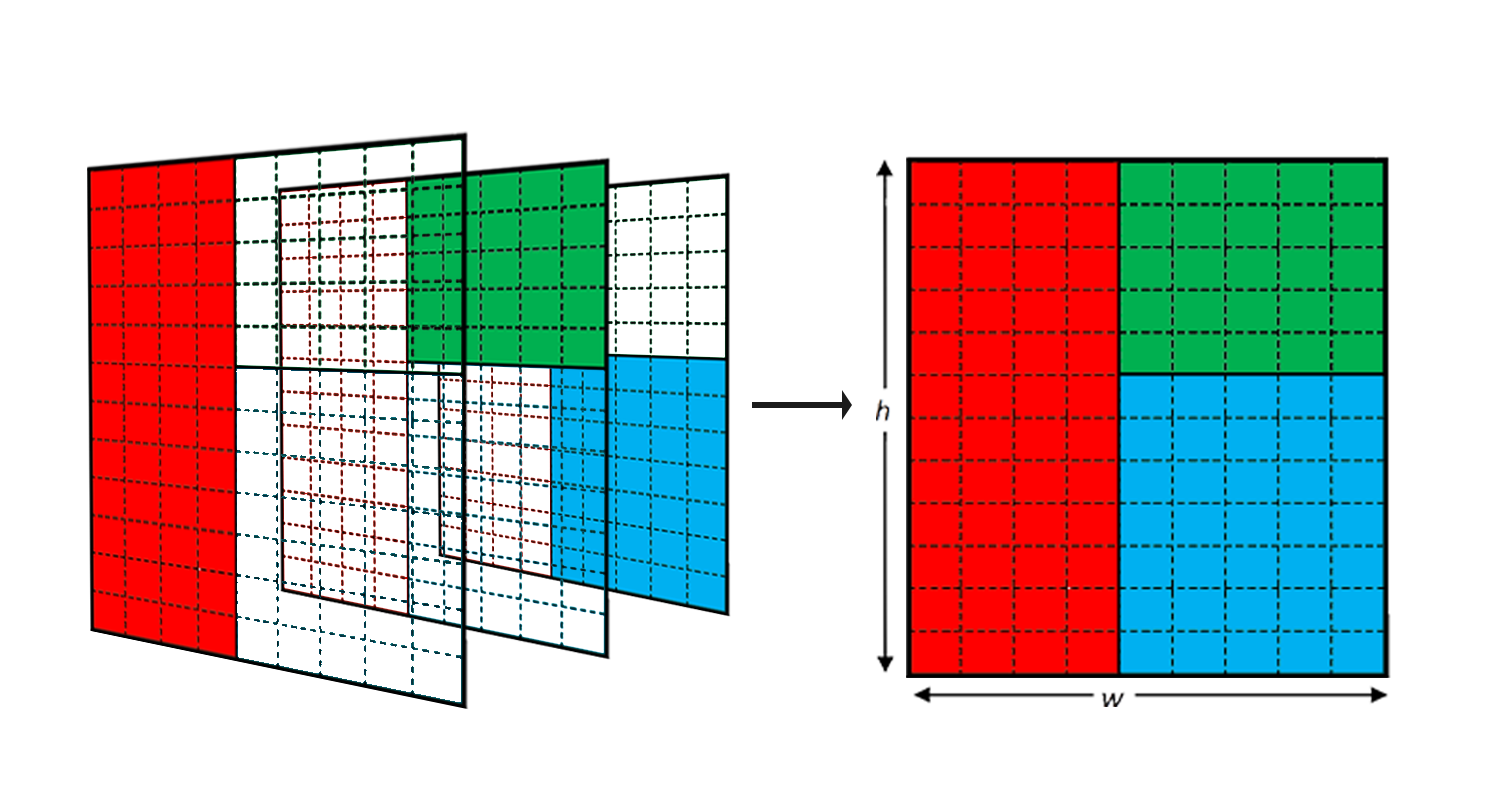
\includegraphics[width=\textwidth]{images/SAT_cube.png}
	\caption{An instance solved with our SAT implementation.}
	\label{fig:overlaps}
\end{figure}

\subsection{Main Problem Constraints}
Now that the problem variables are decided, we can constraint the $Paper$ with some predicates, in \textbf{Propositional Logic}, in order
to carry out the solution of the problem.

\begin{itemize}
    \item[] \textbf{Essential Constraints}
    \item \textbf{\textit{Two different presents must not overlap:}}
    \begin{itemize}
        \item[] Given the two rectangles of two different presents, we can check if they have
            at least one part in common, just by checking if the tensor at position (x, y)
            holds in two different presents i and j. The \textit{overlaps} predicate is defined as:
        \item[] \begin{equation*}\begin{multlined}
            overlaps(Present_1, Present_2) \leftrightarrow \\
            \bigvee_{x, y \in Paper}(Paper[x, y, Present_1] \wedge Paper[x, y, Present_2])
        \end{multlined}\end{equation*}
    \end{itemize}
    \item \textbf{\textit{The presents must have and occupy the correct dimension:}}
    \begin{itemize}
        \item[] This was one of the hardes constrain to develop. We have to force the tensor to have the right
            ammount of true values in the correct place, for each present at a gien coordinate. The idea is
            that given a certain coordinate, we force the tensor to obbey a certain \textit{Disjunctive Normal Formula}.
        \item[] For each present, we fix a tuple of initial coordinates $(x_0, y_0)$ and we force the tensor to hold at 
                all the subsequent $Width \times Height$ coordinates, and not to hold the rest.
                Then we translate the initial coordinates and repeat the extraction of the formula.
                Once we have all the formulas for all the possible initial position of the present in the paper sheet,
                we concatenate them with an Or series into a \textit{Disjunctive Normal Formula}.
                Let's define the following predicate, where $p$ is the index of the current present:
        \item[] \begin{equation*}\begin{multlined}
            correct\_dimension(p, dx, dy) \leftrightarrow \\
            \bigvee_{
                \substack{
                    x_0 \in [1, Width - dx]\\
                    y_0 \in [1, Height - dy]
                }
            }
            (\bigwedge_{
                \substack{
                    x \in [x_0, x_0 + dx] \\
                    y \in [y_0, y_0 + dy]
                }
             } Paper[x, y, p])
             \vee
            (\bigwedge_{
                \substack{
                    x \in [1, x_0] \cup [x_0 + dx + 1, Width]\\
                    y \in [1, y_0] \cup [y_0 + dy + 1, Height]
                }
             } \neg Paper[x, y, p]) 
        \end{multlined}\end{equation*}
        \item[] So we end up with the full constrain:\\
        \begin{equation*} \bigwedge_{p \in [1, Presents]} correct\_dimension(p, Dimension_x[p], Dimension_y[p]) \end{equation*}  
    \end{itemize}
    \item \textbf{\textit{Each tensor tuple of coordinates must have at least one present:}}
    \item[] We want the tensor to have at least one present at each tuple of coordinates $(x, y)$:
    \begin{itemize}
        \item[] \begin{equation*}
            \bigwedge_{
                \substack{
                    x \in [1, Width]\\
                    y \in [1, Height]
                }
            } \bigvee_{p \in [1, Presents]} Paper[x, y, p]
        \end{equation*}
    \end{itemize} 
    \item[] \textbf{Additional Constraints}
    \item[] These constraint are not essential to solve the general formulation of this problem,
        but they results helpful as they restrict the search space in the given instances.
        The underlying assumption is that the instance contains the right amount of presents such
        that the area of the Paper Sheet is completely used.
    \item \textbf{\textit{}}
    \item \textbf{\textit{The presents must fill the row (column) dimension:}}
        \begin{itemize}
            \item[] We want to use each row \textit{(or column)} such that we use all of the available area of the paper.
            \item[] Drawing a vertical \textit{(horizontal)} we check that at least one present holds in the tensor in the line coordinates:
            \item[] Rows: \begin{equation*}\bigvee_{y \in [1, Height]} \bigwedge_{x \in [1, Width]} \bigvee_{p \in [1, Presents]} Paper[x, y, p]\end{equation*}
            \item[] Cols: \begin{equation*}\bigvee_{x \in [1, Width]} \bigwedge_{y \in [1, Height]} \bigvee_{p \in [1, Presents]} Paper[x, y, p]\end{equation*}
        \end{itemize}
\end{itemize}


\begin{center}
    \begin{tabular}{|c|c|r|r|r|}
        \hline
        \multicolumn{5}{|c|}{\textbf{Results - SAT - Base Model}} \\
        \hline
        \textbf{Instance} & \textbf{Time} & \textbf{Nodes} & \textbf{Propagations} & \textbf{Memory \textit{[KB]}} \\
        
        \hline
		8x8 & 00:00:00.024 & 5 & 352 & 3,610 \\ \hline
		9x9 & 00:00:00.047 & 5 & 562 & 4,380 \\ \hline
		10x10 & 00:00:00.030 & 35 & 4,529 & 6,220 \\ \hline
		11x11 & 00:00:00.081 & 131 & 6,394 & 9,110 \\ \hline
		12x12 & 00:00:00.558 & 4,854 & 707,773 & 15,780 \\ \hline
		13x13 & 00:00:00.278 & 10 & 2,339 & 17,860 \\ \hline
		14x14 & 00:00:00.305 & 25 & 3,582 & 20,720 \\ \hline
		15x15 & 00:00:00.419 & 10 & 3,346 & 28,460 \\ \hline
		16x16 & 00:00:01.255 & 7,074 & 1,282,930 & 50,450 \\ \hline
		17x17 & 00:00:00.893 & 11 & 5,421 & 52,210 \\ \hline
		18x18 & 00:00:01.630 & 14 & 8,421 & 100,410 \\ \hline
		19x19 & 00:00:27.630 & 288,683 & 29,385,116 & 186,140 \\ \hline
		20x20 & 00:00:09.644 & 101,838 & 14,410,029 & 180,390 \\ \hline
		21x21 & 00:00:40.285 & 457,133 & 55,916,656 & 286,750 \\ \hline
		22x22 & 00:00:07.482 & 139,013 & 9,572,398 & 281,030 \\ \hline
		23x23 & 00:09:56.789 & 1,962,511 & 534,675,767 & 712,110 \\ \hline
		24x24 & 00:00:03.612 & 19 & 16,426 & 269,930 \\ \hline
		25x25 & 00:05:55.417 & 1,233,566 & 346,485,749 & 775,680 \\ \hline
		26x26 & 00:45:17.499 & 5,767,742 & 1,971,230,196 & 1,496,340 \\ \hline
		27x27 & 00:00:08.523 & 21 & 24,446 & 536,800 \\ \hline
		28x28 & 00:32:35.297 & 4,521,694 & 1,098,468,605 & 1,405,660 \\ \hline
		29x29 & 00:00:12.385 & 24 & 33,032 & 846,010 \\ \hline
		30x30 & 00:00:11.579 & 21 & 29,327 & 775,680 \\ \hline
		31x31 & 00:00:11.336 & 19 & 29,474 & 735,900 \\ \hline
		32x32 & 00:00:22.700 & 25 & 44,554 & 1,224,890 \\ \hline
		33x33 & 00:11:23.633 & 1,656,979 & 440,157,987 & 2,502,960 \\ \hline
		34x34 & 00:00:14.357 & 136 & 43,197 & 1,219,280 \\ \hline
		35x35 & 01:29:31.537 & 5,614,518 & 3,015,411,866 & 3,903,330 \\ \hline
		36x36 & \multicolumn{4}{|c|}{Time $>$ 10h - Max Time Elasped} \\ \hline
		37x37 & \multicolumn{4}{|c|}{Time $>$ 10h - Max Time Elasped} \\ \hline
		38x38 & 00:17:21.723 & 1,507,275 & 214,330,184 & 1,925,140 \\ \hline
		39x39 & 00:03:19.897 & 28 & 76,042 & 3,041,150 \\ \hline
		40x40 & 00:22:13.868 & 899,810 & 115,199,209 & 3,041,150 \\ \hline
		rotation\_test & - & - & - & - \\ \hline

    \end{tabular}
\end{center}


\section{Rotation Model}
As for \textbf{CP} and \textbf{SMT}, we just need another variable that keeps track of the rotation of each presnt in the paper sheet:

In this case, we do not need to use a proxy to gather the correct dimension, we just check the correct dimension in two different ways: the normal or the rotated one.
Like this, we can place each present in the normal \textit{OR} the rotated way and this is the resulting constrain: 
\begin{equation*}\begin{multlined}
    \bigwedge_{p \in [1, Presents]} (\\
        correct\_dimension(p, Dimension_x[p], Dimension_y[p]) \vee\\
        correct\_dimension(p, Dimension_y[p], Dimension_x[p]) \\
    )
\end{multlined}\end{equation*}  

As we can see, by switching the two dimension, we can simply rotate the present.


\begin{center}
    \begin{tabular}{|c|c|r|r|}
        \hline
        \multicolumn{4}{|c|}{\textbf{Results}} \\
        \hline
        \textbf{Instance} & \textbf{Time} & \textbf{Nodes} & \textbf{Propagations} \\
        
        \hline
		8x8 & - & - & - \\ \hline
		9x9 & - & - & - \\ \hline
		10x10 & - & - & - \\ \hline
		11x11 & - & - & - \\ \hline
		12x12 & - & - & - \\ \hline
		13x13 & - & - & - \\ \hline
		14x14 & - & - & - \\ \hline
		15x15 & - & - & - \\ \hline
		16x16 & - & - & - \\ \hline
		17x17 & - & - & - \\ \hline
		18x18 & - & - & - \\ \hline
		19x19 & - & - & - \\ \hline
		20x20 & - & - & - \\ \hline
		21x21 & - & - & - \\ \hline
		22x22 & - & - & - \\ \hline
		23x23 & - & - & - \\ \hline
		24x24 & - & - & - \\ \hline
		25x25 & - & - & - \\ \hline
		26x26 & - & - & - \\ \hline
		27x27 & - & - & - \\ \hline
		28x28 & - & - & - \\ \hline
		29x29 & - & - & - \\ \hline
		30x30 & - & - & - \\ \hline
		31x31 & - & - & - \\ \hline
		32x32 & - & - & - \\ \hline
		33x33 & - & - & - \\ \hline
		34x34 & - & - & - \\ \hline
		35x35 & - & - & - \\ \hline
		36x36 & - & - & - \\ \hline
		37x37 & - & - & - \\ \hline
		38x38 & - & - & - \\ \hline
		39x39 & - & - & - \\ \hline
		40x40 & - & - & - \\ \hline
		rotation\_test & - & - & - \\ \hline

    \end{tabular}
\end{center}


\section{On the hardness of SAT modelling}
There are just a few of the implemented model because we wanted to devolop them just by using the Popositional Logic predicates, without recurring with Arithmetics
and Numerical calculus. We strugled to achieve the implementation of new models, but we have been discouraged by the loss of performance in the \textbf{SMT Symmetry Breaking} models,
so we decided to try to improve as best as possible the basical models.\\
Another weak point for the \textbf{SAT} is that we can't write a general purpose program in \textbf{SMT2Lib} standard. Indeed, to achieve such a generalization, we need to use
numerical calculus, not completely available in the \textbf{Propositional Logic}.\\

Another hard point for the \textbf{SAT} modelling was building up the problem. Indeed, we generate a problem building incremental constraints that grows up exponentially with the size of
the paper sheet, the number of presents and their size, since the \textbf{\textit{``Correct Dimension"}} constraint slide a present over the whole paper sheet. For this reason, it could happen
that the problem construction takes more time then its resolution. The construction process takes in average from 3 to 15 minutes, but for tiny or small instances the resolution time can be lesser
than one minute. At the end of day, this can also be acceptable for big instances, where the resolution time is greater than a minute
\textit{(The given times are measured on the same machine, trying to respect the same conditions)}.

We should also take in account that \texttt{Z3} is still in development and has some unexpected behaviours, especially when it boil down to a time matter.
As many many issues come up, it seems that just by renaming variables the time performance of the solver is influenced \cite{z3issues}.
Our decision was to show a view of the resolution times as like as these issues do not exist, so we intended them as model dependent.

\section{Results}
During the resolution of the statistics we tried different \textbf{Resolution Strategy} for the Z3 Solver:
\begin{itemize}
	\item \texttt{default} strategy
	\item \texttt{Z3\_mk\_solver}
	\item \texttt{Z3\_mk\_simple\_solver}
\end{itemize}
We found that the most suitable and efficient for our problem is \texttt{Z3\_mk\_simple\_solver} that optimizes the resolution times up to 15\%.

We briefly recap the overall results of the previous models in a textual informative table:

\begin{center}
    \begin{tabular}{|c|c|c|c|c|}
        \hline
        \multicolumn{5}{|c|}{\textbf{Global Results}} \\
        \hline
        \textbf{Model} & \textbf{Speed} & \textbf{Complexity} & \textbf{Strengths} & \textbf{Weaknesses} \\
        \hline
    \end{tabular}
\end{center}